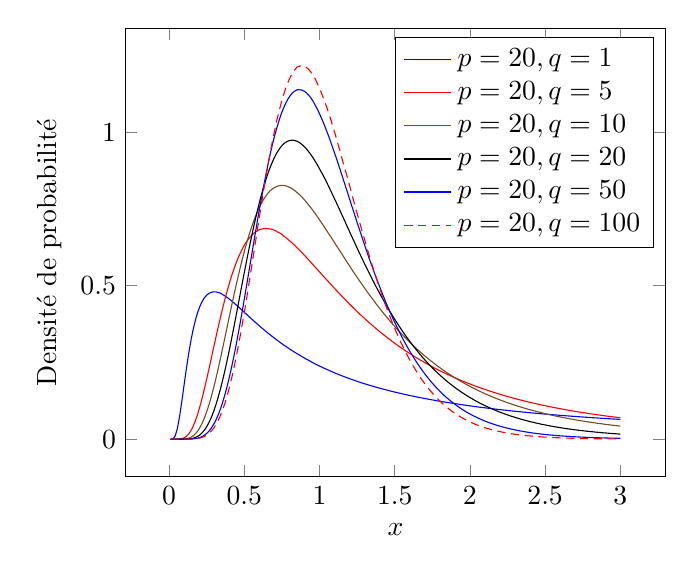
\begin{tikzpicture}[
  declare function={
    gamma(\z)=(2.506628274631*sqrt(1/\z)+ 0.20888568*(1/\z)^(1.5)+ 0.00870357*(1/\z)^(2.5)- (174.2106599*(1/\z)^(3.5))/25920- (715.6423511*(1/\z)^(4.5))/1244160)*exp((-ln(1/\z)-1)*\z);},
  declare function={
    beta(\x,\y)=gamma(\x)*gamma(\y)/gamma(\x+\y);
  },
  declare function={
    fisher(\x,\a,\b) = 1 / beta(\a/2, \b/2) * (\a/\b)^(\a/2) * \x^(\a/2-1) * (1 + \a/\b*\x)^(-(\a + \b)/2);
  }
]
\begin{axis}[
  xlabel = $x$,
  ylabel = {Densité de probabilité},
  samples = 200,
  restrict y to domain = 0:1.5,
  domain = 0.01:3,
  legend cell align=left]
  \foreach \q in {1, 5, 10, 20, 50, 100} {
    \foreach \p in {20} {
      \addplot+[mark={}] {fisher(x,\p, \q}; \addlegendentryexpanded{$p=\p, q=\q$}}}

\end{axis}
\end{tikzpicture}
